\documentclass[a4paper,12pt]{article}
\usepackage[T1]{fontenc} 

%%%%%%%%%%%%%%%%%%%%%%%%%%%%%%%% CONSTANTES %%%%%%%%%%%%%%%%%%%%%%%%%%%%%%%%%%%
\newcommand{\numero}{11}                                    %Numéro de la série -1

\usepackage[french]{babel}
\usepackage[utf8]{inputenc}
\usepackage{answers}

\usepackage{hyperref}
\usepackage{multicol}

\usepackage[table,xcdraw]{xcolor}
\usepackage{listings}
\definecolor{ForestGreen}{RGB}{34,139,34}


\usepackage{enumitem}

\AtBeginDocument{\def\labelitemi{$\bullet$}}


\newcommand{\py}{\lstinline{Python} }


\definecolor{backcolour}{rgb}{0.95,0.95,0.92}

\lstset{%
	language         = Python,
	backgroundcolor  = \color{backcolour},
	basicstyle       = \ttfamily, % \upshape\ttfamily,
	keywordstyle     = \bfseries\color{blue}, %\bfseries,
	stringstyle      = \color{magenta},
	commentstyle     = \color{ForestGreen},
	alsoletter = > ,
	morekeywords = {>>>,as,assert,False,None, nonlocal,True, with,yield , <<, >>, :},
	showstringspaces = false,
	numbers=left,
	stepnumber=1,
	literate={à}{{\`{a}}}1 {é}{{\'e}}1 {è}{{\`{e}}}1 {ê}{{\^{e}}}1 {Ê}{{\^{E}}}1 {î}{{\^i}}1 {ô}{{\^{o}}}1 {ç}{{\c{c}}}1 {Ç}{{\c{C}}}1
}

\newcommand{\itemb}[1]{\item \textbf{#1}}

\usepackage{fancyhdr}  %package pour en-tetes et pied de pages
\usepackage{sectsty} % Permet de faire des modifications de police dans diverses sections des "headings" (cf. modif presentation de la page)
\pagestyle{fancy}       %Style pour en-tetes et pieds de pages
\fancyhead[CO,CE]{\sc Série 1\hspace{0.5mm}}
\fancyhead[RO,LE]{Collège Sismondi}  % LaTeX/TEX define \strut to be an invisible box of width zero that extends just enough above and below the baseline. Cela permet d'augementer légèrement la taille en bas de la box de manière à ce qu'elle soit collée à la ligne.
\fancyhead[LO,RE]{\small\ \textsl{1\textsuperscript{ère} année - DO Informatique}}
\fancyfoot[RO,LE]{2021 - 2022}
\fancyfoot[LO,RE]{\small }
\fancyfoot[CO,CE]{\thepage}

\fancyhfoffset[l]{1.2cm} % le "l" en paramètre permet d'indiquer qu'on ne veut modifier que la marge à gauche.
\renewcommand{\headrule}{{%
		\hrule \headwidth \headrulewidth \vskip-\headrulewidth}}
\renewcommand\footrulewidth{\headrulewidth}
\renewcommand{\footrule}{{%
		\vskip-\footruleskip\vskip-\footrulewidth
		\hrule \headwidth \footrulewidth\vskip\footruleskip}}

\usepackage{tikz}
%-------------------------------------------------------------------------------
%---- Eclairage : en encadré sur fond jaune avec symbôle "ampoule" à gauche ----
%-------------------------------------------------------------------------------
\definecolor{coleclairage}{RGB}{255 , 221 , 156}
\definecolor{contoureclairage}{RGB}{255 , 192 , 0}
\newenvironment{eclairage}
{
	\begin{center}%
		\begin{tikzpicture}%
			\node[rectangle, draw=contoureclairage, top color=coleclairage!50, bottom color=coleclairage!140, rounded corners=5pt, inner xsep=5pt, inner ysep=6pt, outer ysep=10pt]\bgroup                     
			\begin{minipage}{0.98\linewidth}
				\begin{minipage}{0.08\linewidth}\centerline{
\includegraphics[scale=1]{Symbole_eclairage.png}}\end{minipage}
				\begin{minipage}{0.89\linewidth}\itshape\footnotesize
				}
				{                		
				\end{minipage}
			\end{minipage}\egroup;%
		\end{tikzpicture}%
	\end{center}%
}

%-------------------------------------------------------------------------------
%---- apprendre : en encadré sur fond jaune avec symbôle "ampoule" à gauche ----
%-------------------------------------------------------------------------------
\definecolor{colapprendre}{RGB}{50,205,50}
\definecolor{contourapprendre}{RGB}{34,139,34}
\newenvironment{apprendre}
{
	\begin{center}%
		\begin{tikzpicture}%
			\node[rectangle, draw=contourapprendre, top color=colapprendre!10, bottom color=colapprendre!50, rounded corners=5pt, inner xsep=5pt, inner ysep=6pt, outer ysep=10pt]\bgroup                     
			\begin{minipage}{0.98\linewidth}
				\begin{minipage}{0.08\linewidth}\centerline{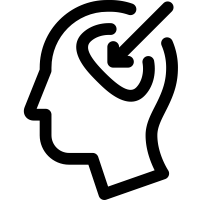
\includegraphics[width=30px]{Symbole_learn.png}}\end{minipage}
				\begin{minipage}{0.89\linewidth}\itshape\footnotesize
				}
				{                		
				\end{minipage}
			\end{minipage}\egroup;%
		\end{tikzpicture}%
	\end{center}%
}

\definecolor{colimportant}{RGB}{247 , 189 , 164}
\definecolor{contourimportant}{RGB}{237 , 125 , 49}
\newenvironment{important}
{
	\begin{center}%
		\begin{tikzpicture}%
			\node[rectangle, draw=contourimportant, top color=colimportant!50, bottom color=colimportant!140, rounded corners=5pt, inner xsep=5pt, inner ysep=6pt, outer ysep=10pt]\bgroup                     
			\begin{minipage}{0.08\linewidth}\centerline{
\includegraphics[scale=0.8]{Symbole_attention.png}}\end{minipage}
			\begin{minipage}{0.89\linewidth}
			}
			{                		
			\end{minipage}\egroup;
		\end{tikzpicture}%
	\end{center}%
}

%-----------------------------------------------------------------
%---- Modification présentation de la page: marges de la page ----
%-----------------------------------------------------------------
%\addtolength{\hoffset}{-1in}              % 1
%\addtolength{\voffset}{-1in}              % 2
\addtolength{\oddsidemargin}{-0.1 in} % 3
\addtolength{\evensidemargin}{-1in} % 3
\addtolength{\topmargin}{-1in}       % 4
\addtolength{\headheight}{6pt}       % 5
%\addtolength{\headsep}{-0.2cm}           % 6
\setlength{\textheight}{26cm}    % 7
\setlength{\textwidth}{16.5cm}      % 8
\addtolength{\marginparsep}{0pt}      % 9
\setlength{\marginparwidth}{0pt}   % 10
\addtolength{\footskip}{-1mm}           %11

\setlength{\parindent}{0em}% pas d'indentation


% Customiser le nom des sections
\usepackage{titlesec}
\titleformat{\section}[hang]{\Large \bfseries}{Série \thesection:\ }{0pt}{}

\renewcommand{\familydefault}{\sfdefault} % pour avoir des polices san serif

\newtheorem{Exc}{Exercice}
\Newassociation{correction}{Soln}{mycor}
\renewcommand{\Solnlabel}[1]{\bfseries Ex #1 }
\def\exo#1{%
	\futurelet\testchar\MaybeOptArgmyexoo}
\def\MaybeOptArgmyexoo{
	\ifx[\testchar \let\next\OptArgmyexoo
	\else \let\next\NoOptArgmyexoo \fi \next}
\def\OptArgmyexoo[#1]{%
	\begin{Exc}[#1]\normalfont}
	\def\NoOptArgmyexoo{%
		\begin{Exc}\normalfont}
		\newcommand{\finexo}{\end{Exc} \vspace{3mm}}
	\newcommand{\flag}[1]{}
	\newcommand{\entete}[1]

\newcommand{\getexocompteur}{{\the\numexpr \arabic{Exc}  \relax}}	
	
\newcommand{\eexo}{\vspace{5mm}} % espace pour séparer les exercices
\definecolor{light-gray}{gray}{0.95} 
\lstset{language=Python, upquote=true, showstringspaces=false, columns=fullflexible, basicstyle = \ttfamily, backgroundcolor = \color{light-gray}, numbers=right, stepnumber=1, keywordstyle=\color{blue}, stringstyle=\color{magenta}, commentstyle=\color{red}, breaklines=true,} 

\begin{document}
%		\title{\vspace{-3cm}Série 1}
%		\date{\vspace{-2cm}}
%		\maketitle

\fancyhead[CO]{\sc Série \arabic{section} \hspace{0.5mm}}
%\fancyhead[CE]{\sc Série \arabic{section} \hspace{0.5mm}}
\setcounter{section}{\numero}

\section{Structure de contrôle et utilisation de fonctions}
\Opensolutionfile{mycor}[cor01]
%%%%%%%%%%%%%%%%%%%%%%%%%%%%%%%% EXERCICE %%%%%%%%%%%%%%%%%%%%%%%%%%%%
\exo{}[Compréhension de code]  ~\\ 
\begin{lstlisting}
n = 4
for i in range(n):
    print(i)
\end{lstlisting}
Que va afficher ce code Python ?
\begin{lstlisting}https://www.overleaf.com/project/614b7a33668562d2ad26e0cd
n = 4
for i in range(2, n):
    print(i)
\end{lstlisting}
Et celui-ci ?
\begin{correction}
		~\\ \vspace{-5pt}
		Le premier exemple affichera successivement les valeurs 1, 2 et 3.
		
		Le second affichera uniquement 2 et 3.
	\end{correction}
\finexo
%%%%%%%%%%%%%%%%%%%%%%%%%%%%%%%% EXERCICE %%%%%%%%%%%%%%%%%%%%%%%%%%%%
\exo{}[Compréhension de code]  ~\\ 
Voici un code en Python:
\begin{lstlisting}
x = 1
for i in range(4):
    x = x + i
\end{lstlisting}
Quelle est la valeur finale de x ?
\begin{correction}
		~\\ \vspace{-5pt}
		%\\lstinputlisting[numbers=none]{codes/corr_exo_verif_age.py}
		La variable i prend successivement les valeurs 0, 1, 2 et 3. Donc x prend les valeurs 1, 2, 4 et 7.
\end{correction}
\finexo
%%%%%%%%%%%%%%%%%%%%%%%%%%%%%%%% EXERCICE %%%%%%%%%%%%%%%%%%%%%%%%%%%%
\exo{}[Compréhension de code]  ~\\ 
Voici une fonction définie en Python:
\begin{lstlisting}
def f(x):
    for d in range(2, x):
        if x % d == 0:
            return d
\end{lstlisting}
Que renvoie la fonction f si le paramètre x a la valeur 15 ?
\begin{correction}
		~\\ \vspace{-5pt}
		%\\lstinputlisting[numbers=none]{codes/corr_exo_verif_age.py}
		Le nombre 15 est divisible par 3, donc la fonction renvoie 3. Ce retour interrompt le code.
\end{correction}
\finexo
%%%%%%%%%%%%%%%%%%%%%%%%%%%%%%%% EXERCICE %%%%%%%%%%%%%%%%%%%%%%%%%%%%
\exo{}[Compréhension de code]  ~\\ 
Que va afficher le code suivant ?
\begin{lstlisting}
compteur = 0
while compteur < 12:
    if(compteur%3)==0:
        print("Zig")
    elif(compteur%3)==1:
        print("Zag")
    elif(compteur%3)==2:
        print("Zoug")
    compteur += 1
\end{lstlisting}
\begin{correction}
Le résultat sera affiché sera:
\begin{lstlisting}
Zig
Zag
Zoug
Zig
Zag
Zoug
Zig
Zag
Zoug
Zig
Zag
Zoug
\end{lstlisting}
\end{correction}
\finexo
%%%%%%%%%%%%%%%%%%%%%%%%%%%%%%%% EXERCICE %%%%%%%%%%%%%%%%%%%%%%%%%%%%
\exo{}[Compréhension de code]  ~\\ 
Que va afficher le code suivant si vous vous prénommez Cindy ?
\begin{lstlisting}
texte_debut = "Bonjour"
texte_fin = "Au revoir"
prenom = input("Quel est votre prénom ? : ")
for i in range(4):
    print(texte_debut, prenom + ".")
    if i == 3 :
        print(texte_fin, prenom + ".")
\end{lstlisting}
\begin{correction}
Le résultat sera affiché sera:
\begin{lstlisting}
Bonjour Cindy.
Bonjour Cindy.
Bonjour Cindy.
Bonjour Cindy.
Au revoir Cindy.
\end{lstlisting}
	\end{correction}

\finexo
%%%%%%%%%%%%%%%%%%%%%%%%%%%%%%%% EXERCICE %%%%%%%%%%%%%%%%%%%%%%%%%%%%
\exo{}[Compréhension de code]  ~\\ 
Après le code Python qui suit, quelles sont les valeurs finales de x et de y ?
\begin{lstlisting}
x = 4
while x > 0:
    y = 0
    while y < x:
        y = y + 1
        x = x - 1
\end{lstlisting}
\begin{correction}
		~\\ \vspace{0pt}
		%\\lstinputlisting[numbers=none]{codes/corr_exo_verif_age.py}
Les valeurs de x sont strictement décroissantes et la valeur de y est remise à 0 dès qu'elle n'est plus strictement inférieure à celle de x. Au dernier passage dans la boucle interne, y vaut 0, et x vaut 1 : y prend alors la valeur de 1 et x la valeur de 0;
on sort de la boucle interne puis de la boucle externe.
On a une boucle infinie si on remplace y=0 par y=1.
\end{correction}

\finexo
%%%%%%%%%%%%%%%%%%%%%%%%%%%%%%%% EXERCICE %%%%%%%%%%%%%%%%%%%%%%%%%%%%
\exo{}[Compréhension de code]  ~\\ 
Analysez le script ci-dessous et indiquez ce qui sera affiché.
\begin{lstlisting}
# definition de la fonction
def table_7():
    for n in range(1, 13):
        print(n*7, end=' ')
    
# appel de la fonction
table_7()
\end{lstlisting}
\begin{correction}
		~\\ \vspace{-5pt}
		%\\lstinputlisting[numbers=none]{codes/corr_exo_verif_age.py}
La variable n prend successivement les valeurs de 1 à 12.
Le résultat sera affiché sera:
\begin{lstlisting}
7 14 21 28 35 42 49 56 63 70 77 84 
\end{lstlisting}
end=' '  dans la fonction print indique de ne pas aller à la ligne et de séparer chaque print(n*7) par un espace.
	\end{correction}

\finexo
%%%%%%%%%%%%%%%%%%%%%%%%%%%%%%%% EXERCICE %%%%%%%%%%%%%%%%%%%%%%%%%%%%
\exo{}[Erreur de syntaxe]  ~\\ 
Chacun des scripts ci-dessous contient une erreur de syntaxe différente. Laquelle ? Après avoir deviné, vous pouvez tester en mode interactif : soyez attentifs au message d’erreur affiché !
\begin{lstlisting}
def table_7()
    for n in range(13):
        print(n*7,end=' ')
\end{lstlisting} 
\begin{lstlisting}           
def table_7:
    for n in range(13):
        print(n*7,end=' ')        
\end{lstlisting} 
\begin{lstlisting}   
table_7():
    for n in range(13):
        print(n*7,end=' ')
\end{lstlisting} 
\begin{lstlisting}       
def table_7():
for n in range(13):
    print(n*7,end=' ')
\end{lstlisting}
\begin{correction}
	~\\ \vspace{-5pt}
	%\\lstinputlisting[numbers=none]{codes/corr_exo_verif_age.py}
	\begin{enumerate}
        \item Il manque \lstinline{:} après \lstinline{def table_7()}
        \item Il manque \lstinline{()} entre \lstinline{table_7 et :}
        \item Il manque \lstinline{def} au début de la fonction \lstinline{table_7():}
        \item la boucle \lstinline{for} n'est pas indentée correctement dans la fonction.
    \end{enumerate}
\end{correction}
\finexo
\newpage
%%%%%%%%%%%%%%%%%%%%%%%%%%%%%%%% EXERCICE %%%%%%%%%%%%%%%%%%%%%%%%%%%%
\exo{}[Les différences]  ~\\ 
Analysez les deux scripts suivants : quelles sont les différences ? Constatez-vous une ou plusieurs erreurs de programmation ?
\begin{lstlisting}
def est_pair(n):
    if n % 2 == 0:
        print('True')
    else:
        print('False')

nombre = 14
if not est_pair(nombre):
    print(nombre,' est impair')
else:
    print(nombre,' est pair')
\end{lstlisting} 
\begin{lstlisting}  
def est_pair(n):
    if n % 2 == 0:
        return True
    else:
        return False

nombre = 14
if not est_pair(nombre):
    print(nombre,' est impair')
else:
    print(nombre,' est pair')
\end{lstlisting}
Est-ce que le code de la 2ème fonction peut être simplifiée ? Si oui comment ?
\begin{correction}
	~\\ \vspace{-5pt}
	%\\lstinputlisting[numbers=none]{codes/corr_exo_verif_age.py}
	\begin{enumerate}
        \item Dans le 1er code, la fonction \lstinline{est_pair} ne retourne pas de valeur codée. La fonction retourne par défaut \lstinline{None}. Le programme affichera \lstinline{True} ensuite \lstinline{14 est impair} ce qui est faux !
        \item Le 2ème code est correct.
        \item Oui, la fonction peut être simplifiée.
    \end{enumerate}
\begin{lstlisting}  
def est_pair(n):
    if n % 2 == 0:
        return True
    return False
\end{lstlisting}
Il n'est pas nécessaire d'ajouter le bloc \lstinline{else:} car l'instruction \lstinline{return True} interrompt l’exécution de la fonction ! Mais il est encore possible de simplifier en retournant directement l'évaluation du test \lstinline{n % 2 == 0} qui est soit True, soit False. Notez que les parenthèses ne sont pas nécessaire pour encadrer l'expression évaluée.
\begin{lstlisting}  
def est_pair(n):
    return n % 2 == 0
\end{lstlisting}

\end{correction}

\finexo

%%%%%%%%%%%%%%%%%%%%%%%%%%%%%%%% EXERCICE %%%%%%%%%%%%%%%%%%%%%%%%%%%%
\exo{}[Les paramètres]  ~\\ 
On peut aussi passer à la fonction une liste de {\it paramètres}. Analysez le script ci-dessous et indiquez son résultat.
\begin{lstlisting}
# definition de la fonction    
def tableMulti(base, debut, fin):
    for n in range(debut, fin+1):
        print(n*base, end=' ')

# appel de la fonction
tableMulti(8, 13, 17)
\end{lstlisting}
\begin{correction}
	~\\ \vspace{-5pt}
	%\\lstinputlisting[numbers=none]{codes/corr_exo_verif_age.py}
    Les nombres suivants seront affichés:
    \lstinline{104 112 120 128 136}
\end{correction}
\finexo

\newpage
%%%%%%%%%%%%%%%%%%%%%%%%%%%%%%%% EXERCICE %%%%%%%%%%%%%%%%%%%%%%%%%%%%
\exo{}[Variables locales - variables globales]  ~\\ 
En fonction du point d'exécution d'un programme, la visibilité des variables n'est pas la même: les variables définies dans le contexte de base sont dites globales, les variables définies dans une fonction sont locales.

Donner le résultat ou l'erreur affiché pour les deux codes suivants:
\begin{lstlisting}
a = 1
b = 2
def test(a,b):
    a = 5
    print(a,b)

test(3,4)
print(a,b)
\end{lstlisting} 

\begin{lstlisting}
a = 1
b = 2
def test(a,b):
    print(a,b)
    
def test2(c,d):
    print(a,b)
    
def test3():
    c = 3
    d = 4

test(a,b)
test2(3,4)
test3()
print(c,d)
\end{lstlisting}
\begin{correction}
	~\\ \vspace{-5pt}
	%\\lstinputlisting[numbers=none]{codes/corr_exo_verif_age.py}
    Premier programme, les nombres suivants seront affichés:
   \begin{lstlisting}
   5 4
   1 2
   \end{lstlisting}
    Deuxième programme, les nombres suivants seront affichés:
   \begin{lstlisting}
   1 2
   1 2
    ... Erreur: c n'est pas définie...
       print(c,d)
   NameError: name 'c' is not defined
   \end{lstlisting}

\end{correction}


\finexo

% Solution		
		\newpage
		\setcounter{page}{1}
		\setcounter{section}{\numero}
		\Closesolutionfile{mycor}
		\titleformat{\section}[hang]{\Large \bfseries}{Corrigé Série \thesection:\ }{0pt}{}
		

		\fancyhead[CO]{\sc Corrigé Série \arabic{section} \hspace{0.5mm}}
		\section{}
		\Readsolutionfile{mycor}
	\end{document}